\let\negmedspace\undefined
\let\negthickspace\undefined
\documentclass[journal]{IEEEtran}
\usepackage[a5paper, margin=10mm, onecolumn]{geometry}
\usepackage{tfrupee} 

\setlength{\headheight}{1cm} 
\setlength{\headsep}{0mm}     

\usepackage{gvv-book}
\usepackage{gvv}
\usepackage{cite}
\usepackage{amsmath,amssymb,amsfonts,amsthm}
\usepackage{algorithmic}
\usepackage{graphicx}
\usepackage{textcomp}
\usepackage{xcolor}
\usepackage{txfonts}
\usepackage{listings}
\usepackage{enumitem}
\usepackage{mathtools}
\usepackage{gensymb}
\usepackage{comment}
\usepackage[breaklinks=true]{hyperref}
\usepackage{tkz-euclide} 
\usepackage{listings}                                        
\def\inputGnumericTable{}                                 
\usepackage[latin1]{inputenc}                                
\usepackage{color}                                            
\usepackage{array}                                            
\usepackage{longtable}                                       
\usepackage{calc}                                             
\usepackage{multirow}                                         
\usepackage{hhline}                                           
\usepackage{ifthen}                                           
\usepackage{lscape}

\begin{document}

\bibliographystyle{IEEEtran}
\vspace{3cm}

\title{1.6.23}
\author{AI25BTECH11008 - Chiruvella Harshith Sharan}
{\let\newpage\relax\maketitle}

\renewcommand{\thefigure}{\theenumi}
\renewcommand{\thetable}{\theenumi}
\setlength{\intextsep}{10pt} 

\numberwithin{equation}{enumi}
\numberwithin{figure}{enumi}
\renewcommand{\thetable}{\theenumi}

\textbf{Question}: Find the direction cosines of the line joining points \textbf{P} (4, 3, -5)\\ \hspace*{1.2cm} and \textbf{Q} (-2, 1, 8).\\\\

\textbf{Question}: Find the direction cosines of the line joining points 
\textbf{P}(4,3,-5) and \textbf{Q}(-2,1,8). \\\\[0.3cm]

\textbf{Solution}: \\\\[0.3cm]

The direction vector of the line is
\[
\vec{PQ} = \vec{Q} - \vec{P} 
= \myvec{-2 \\ 1 \\ 8} - \myvec{4 \\ 3 \\ -5}
= \myvec{-6 \\ -2 \\ 13}.
\]

\vspace{0.3cm}

The magnitude of this vector is
\[
|\vec{PQ}| = \sqrt{(-6)^2 + (-2)^2 + (13)^2}
= \sqrt{36+4+169}
= \sqrt{209}.
\]

\vspace{0.3cm}

Hence, the direction cosines are
\[
l = \frac{-6}{\sqrt{209}}, \quad 
m = \frac{-2}{\sqrt{209}}, \quad 
n = \frac{13}{\sqrt{209}}.
\]

\vspace{0.3cm}

Thus, the direction cosines of the line are
\[
\myvec{\tfrac{-6}{\sqrt{209}} \\[6pt] \tfrac{-2}{\sqrt{209}} \\[6pt] \tfrac{13}{\sqrt{209}} }.
\]

\begin{figure}[htbp]
    \centering
    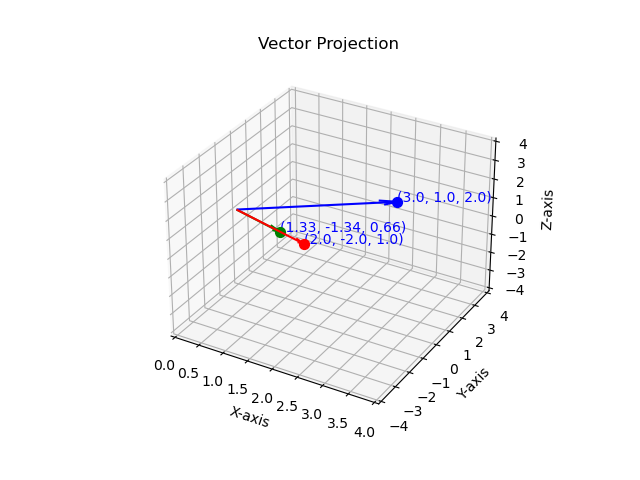
\includegraphics[width=0.8\linewidth]{figs/fig1.png}
    \caption{Graph showing collinear points A, B, C}
    \label{fig:fig/fig1.png}
\end{figure}

\end{document}
